%TC:ignore

% to ignore textcount.

\documentclass[]{article}

\usepackage{graphicx}
\usepackage{amsmath}
\usepackage{textcomp}
\usepackage{siunitx}
\usepackage{geometry}
\usepackage[table]{xcolor}
\usepackage{nicefrac}
\usepackage{siunitx}
\usepackage[english]{babel}
\usepackage[nottoc,numbib]{tocbibind}
\usepackage[autostyle]{csquotes}
\usepackage[
	backend=biber,
	citestyle=apa,
	bibencoding=utf8,
	style=apa,
	sortlocale=en_US,
	uniquename=false,
	url=true, 
	doi=true,
	eprint=false
]{biblatex}
\addbibresource{zoterolibrary.bib}
\usepackage{hyperref}
\hypersetup{colorlinks=true}
\usepackage[doublespacing]{setspace}
\usepackage{booktabs}
\usepackage{doi}
\usepackage[flushleft]{threeparttable}
\usepackage{authblk}
\usepackage[switch]{lineno}
\linenumbers
\usepackage{xr}


% \usepackage[acronym, toc]{glossaries-extra}
\usepackage[acronym]{glossaries-extra}
\glsdisablehyper
\setabbreviationstyle{long-short}
\newabbreviation{es}{ES}{ecosystem service}

\usepackage{textcomp}
\newcommand{\textapproxx}{\raisebox{0.5ex}{\texttildelow}}


\makeatletter
\newcommand*{\addFileDependency}[1]{% argument=file name and extension
  \typeout{(#1)}
  \@addtofilelist{#1}
  \IfFileExists{#1}{}{\typeout{No file #1.}}
}
\makeatother

\newcommand*{\myexternaldocument}[1]{%
    \externaldocument{#1}%
    \addFileDependency{#1.tex}%
    \addFileDependency{#1.aux}%
}




\DeclareSourcemap{
	\maps[datatype=bibtex, overwrite]{
		% otherwise my annotations from Mendeley/Zotero will be shown in the references.
		\map{
			\step[fieldset=annote, null]
		}
		% Replaces '&' with '\&'
		\map{
		% Zotero seems to escape & in the publisher field.
%			\step[fieldsource=publisher, match=\regexp{\x{26}}, replace=\regexp{\\\x{26}}]
%			\step[fieldsource=abstract, match=\regexp{\x{26}}, replace=\regexp{\\\x{26}}]
%			\step[fieldsource=journal, match=\regexp{\x{26}}, replace=\regexp{\\\x{26}}]
%			\step[fieldsource=journaltitle, match=\regexp{\x{26}}, replace=\regexp{\\\x{26}}]
%			\step[fieldsource=title, match=\regexp{\x{26}}, replace=\regexp{\\\x{26}}]
%			\step[fieldsource=note, match=\regexp{\x{26}}, replace=\regexp{\\\x{26}}]
		}
		% for some reason I need this now because abstracts and titles could contain a percentage sign and that breaks everything.
		\map{
			\step[fieldsource = abstract, match = \regexp{([^\\])\%}, replace = \regexp{$1\\\%}]
			\step[fieldsource = title, match = \regexp{([^\\])\%}, replace = \regexp{$1\\\%}]
		}
	}
}

%
%
%
\myexternaldocument{supplements}


%\setstretch{0.75}

\usepackage{xfp}


\DeclareSIUnit\year{yr}

\usepackage[font=scriptsize,labelfont=bf]{caption}

\geometry{
	a4paper,
	total={170mm,257mm},
	left=20mm,
	top=20mm,
}

\newcommand{\coo}{\ensuremath{\mathrm{CO_2}}}

\DeclareUnicodeCharacter{202F}{KG BROKEN CHARACTER!!!!}



\title{Reconciling the EU forest, biodiversity, and climate strategies}


%TC:endignore


\begin{document}





%TC:ignore


\author[1,*]{Konstantin Gregor}
\author[2]{Christopher P.O. Reyer}
\author[3]{Thomas A. Nagel}
\author[4, 5]{Annikki Mäkelä}
\author[1]{Andreas Krause}
\author[1]{Thomas Knoke}
\author[1]{Anja Rammig}

	\affil[1]{TUM School of Life Sciences, Technical University of Munich, Freising, Germany}
	\affil[2]{Potsdam Institute for Climate Impact Research, Member of the Leibniz Association, Potsdam, Germany}
	\affil[3]{University of Ljubljana, Department of Forestry and Renewable Forest Resources, Biotechnical Faculty, 1000 Ljubljana, Slovenia}
	\affil[4]{Department of Forest Sciences, University of Helsinki, Latokartanonkaari 7, Helsinki, Finland}
    \affil[5]{Institute for Atmospheric and Earth System Research / Forest Sciences, Faculty of Agriculture and Forestry, University of Helsinki, Finland}
	\affil[*]{Corresponding author, konstantin.gregor@tum.de}

\date{} 
\setcounter{Maxaffil}{0}


\maketitle




\begin{abstract}
Forests provide important ecosystem services, including climate change mitigation, local climate regulation, habitat for biodiversity, wood and non-wood products, energy, and recreation.
Simultaneously, forests are increasingly affected by climate change and need to be adapted to future environmental conditions.
Current legislation, including the EU Biodiversity Strategy, EU Forest Strategy, and national laws, aims at protecting forest landscapes, enhancing ecosystem services, adapting forests to climate change, and leveraging forest products for climate change mitigation and the bio-economy.
However, reconciling all these competing demands poses a tremendous task for policy-makers, forest managers, conservation agencies, and other stakeholders, especially given the uncertainty associated with future climate impacts.

Here, we used process-based ecosystem modeling and robust multi-criteria optimization to develop forest management portfolios that provide multiple ecosystem services across a wide range of climate scenarios. We included constraints to both strictly protect 10\% of Europe's land area and to provide stable harvest levels under every climate scenario.
The optimization showed that there were limited options to improve ecosystem service provision within these constraints.
Consequently, management portfolios suffered from low diversity, which contradicts the goal of multi-functionality and exposes regions to significant risk due to a lack of risk diversification. Additionally, certain regions, especially those in the north, would need to prioritize timber provision to compensate for reduced harvests elsewhere. This conflicts with EU LULUCF targets for increased forest carbon sinks in all member states and prevents an equal distribution of strictly protected areas, introducing a bias as to which forest ecosystems are more protected than others. Thus, coordinated strategies at the European level are imperative to address these challenges effectively.

We suggest that the implementation of the EU Biodiversity Strategy, EU Forest Strategy, and targets for forest carbon sinks require complementary measures to alleviate the conflicting demands on forests.
\end{abstract}


%TC:endignore


\noindent\textbf{Keywords:} Forest management, climate change mitigation, substitution effects, ecosystem services, robust optimization, carbon sink, Europe, management portfolios


% final revision: 7298 words before last comment of CR implemented.
% intro, methods, results: 7144 (also including abbrev of ES everywhere)
% ton nagel comments: 7091
% before reworking conclusion: 7077

\section{Introduction}

Climate change and biodiversity loss are among humanity's most pressing issues \parencite{IPCCsynthesisAR62023, IPBES2019}. The progress in climate change mitigation has been slow and has fallen short of targets set by the Paris Agreement \parencite{UN2023}. Nevertheless, there is a growing trend worldwide to enact legislation addressing climate change \parencite{Eskander2020}. Likewise, biodiversity loss is continuing at an alarming rate. But despite international policy efforts, it often receives less attention than climate change \parencite{Barbier2018}, sometimes overshadowing the intricate relationship between the two issues \parencite{Sage2020, Portner2023}. On the one hand, a significant portion of biodiversity loss is linked to rising temperatures. Thus, limiting global warming is crucial for preserving biodiversity \parencite{Ohashi2019, Warren2018}.
On the other hand, future land use changes stemming from mitigation policies can be detrimental to biodiversity \parencite{Ohashi2019, Hof2018}.
%Furthermore, present levels of investments in biodiversity conservation are insufficient, despite the fact that future benefits of such conservation efforts far outweigh their costs \parencite{Barbier2018, Knoke2023}.
Hence, there is a clear need for more concrete actions and legislative measures to support biodiversity conservation, especially in Europe, where over 80\% of the land surface have been transformed over the past millennia \parencite{EEALandUse2023, Ellis2021}.


To combat biodiversity loss, the European Union (EU) created the \textit{EU Biodiversity Strategy for 2030} \parencite{EuropeanCommissionBiodivStrat2020}.
Key objectives include the protection of 30\% of its land area by 2030, with 10\% strictly protected, the planting of 3 billion trees, and the establishment of ecological corridors.
``Protection'' refers to responsible management and the prevention of deterioration. Protected forests can be managed for timber, but harvest levels are typically subject to restrictions \parencite{Verkerk2014}.
``Strict protection'' means maintaining ecosystems in an unmanaged state, with interventions limited to those sustaining natural processes \parencite[e.g., wildlife population control,][]{EUProtectionGuidance2022}.
At present, 26\% of the EU's land area are legally protected, and 3\% strictly protected \parencite{EuropeanCommissionBiodivStrat2020, FORESTEUROPE2020}.
Since 35\% of Europe is covered with forests and most other land covers are more intensively used than forests, a substantial portion of newly protected areas will lie in forests \parencite{Hengl2018, FORESTEUROPE2020}.
In addition, the \textit{New EU Forest Strategy for 2030} was proposed, promoting broad-leaved species, forest multi-functionality, carbon sequestration and long-lived wood products, synergies between wood production and conservation, and forest adaptation to climate change \parencite{EUForestStrategy2030}.
Such forward-looking objectives are also often subsumed under the term ``climate-smart forestry'' \parencite{Nabuurs2018}.
Furthermore, both strategies demand the strict protection of Europe's remaining old-growth and primary forests.
Non-EU states have similar strategies in place \parencite[e.g.,][]{UKbiodiv2023, SwissBiodiv2012}.


Managed forests are critical for the European economy, providing income, jobs, and essential resources \parencite{FORESTEUROPE2020}.
The demand for wood products has recently been growing \parencite{Nabuurs2007, FAOSTAT2022, FAO2022}, and further increases are likely, also driven by the transition to a bioeconomy \parencite{Hurmekoski2022}.
Forests also contribute to climate change mitigation through the forest and product carbon sink, and by substituting carbon-intensive non-wood products \parencite[e.g.,][]{Grassi2021}. Additionally, woody bioenergy plays a key role in Europe's energy transition \parencite{EUForestStrategy2030}.
Furthermore, forests offer numerous important \glspl{es}, including biodiversity preservation, local climate regulation, water cycling, and recreation.

The corresponding complex demands placed on forests result in intricate trade-offs. Particularly, the relationships among biodiversity protection, timber production, mitigation, and adaptation, have been extensively discussed in the scientific literature. Most studies indicate a conflict between biodiversity protection and timber production \parencite{Gutsch2018, Verkerk2014b, Felton2016, Baskent2023}, although some suggest synergies \parencite{Biber2020}. Additionally, there is an ongoing debate regarding the mitigation potential of intensively managed, extensively managed, and unmanaged forests \parencite{gregorQuantifyingImpactKey2024, Dugan2018, Soimakallio2021, Gustavsson2021, Petersson2022, Schulte2022, Roebroek2023, Peng2023}.


One potential strategy to address these trade-offs is regional specialization, focusing on wood production in highly productive regions \parencite[e.g.,][]{LessaDerciAugustynczik2021}. This \emph{land sparing} approach allows for increased production in one region while setting aside land for conservation elsewhere \parencite{Balmford2021}. In Europe, however, \emph{land sharing} typically prevails, where both production and protection objectives are pursued on the same land \parencite{Betts2021}, but this could interfere with \textit{strict} protection goals.


Developing forward-looking forest management strategies is a challenging task.
One approach is to use management portfolios, as demonstrated by \textcite{Luyssaert2018}, who optimized portfolios for single objectives, such as maximizing carbon sequestration. Assessing multi-functionality on the other hand, i.e., the provision of multiple \glspl{es}, has been explored by \textcite{Diaz-Balteiro2017}, who selected optimal forest management types for various climate scenarios to find the single best management option in a case study in Spain. Here, we combine the two approaches by developing portfolios for multi-functionality under climate change.


The task is further complicated by the vulnerability of forests to different degrees of climate change and associated disturbances \parencite{Spinoni2018, ipcc_summary_2013, Senf2021, Senf2021a}. Consequently, it is necessary to assess various forest functions under a range of climate scenarios to develop strategies for climate-adapted, multi-functional forests today. Robust multi-criteria optimization offers a valuable tool for this purpose  \parencite{BenTal2002, Groetzner2022, Uhde2017, Ishizaka2013a, Knoke2016}.
\textcite{Gregor2022} employed this approach to compute forest management portfolios for Europe, ensuring the provision of various \glspl{es} across a wide range of climate scenarios. They found that significant portions of unmanaged forests and a gradual transition to more broad-leaved species are beneficial for multi-functional forest landscapes in the face of climate change. However, this would also lead to strong reductions in wood harvests, conflicting with rising wood demands and the objective of leveraging wood products for climate change mitigation.


Here, we investigate to which extent reconciling targets for forest protection, wood production, mitigation, and the provision of \glspl{es} is feasible. We enhanced the methodology of \textcite{Gregor2022} by incorporating Europe-wide constraints on harvest levels and forest protection that must be met under all climate scenarios. Specifically, we explored whether strategies for multi-functional forests can align with stable wood production and the EU's legal aims for strict forest protection and carbon sequestration. Furthermore, we examined the resulting impacts of these constraints on other \glspl{es} and the diversity of management strategies. We considered how the burden imposed by these constraints can be equitably distributed among regions, in line with the directive that all member states should contribute their ``fair share of the effort'' \parencite{EuropeanCommissionBiodivStrat2020}.







%%%%%%%%%%%%%%%%%%%%%%%%%%%%%%%%%%%%%%%%%%%%%%%%%%%%%%%%%%%%%%%%%%%%%%%
%%%%%%%%%%%%%%%%%%%%%%%%%%%%%%%%%%%%%%%%%%%%%%%%%%%%%%%%%%%%%%%%%%%%%%%
%%%%%%%%%%%%%%%%%%%%  METHODS
%%%%%%%%%%%%%%%%%%%%%%%%%%%%%%%%%%%%%%%%%%%%%%%%%%%%%%%%%%%%%%%%%%%%%%%
%%%%%%%%%%%%%%%%%%%%%%%%%%%%%%%%%%%%%%%%%%%%%%%%%%%%%%%%%%%%%%%%%%%%%%%



\section{Methods}

\glsresetall


In this study, building upon simulations with a dynamic vegetation model, we computed forest management portfolios that provide multiple \glspl{es} in an optimally balanced way, while considering the uncertainty of future climate.
In previous work, this optimization was carried out independently for each grid cell \parencite{Gregor2022}, providing one management portfolio suitable for all emission scenarios (Fig. \ref{fig:optimization}).
%In that study, additional hard constraints for the optimization were included, namely restricting the solutions to those where future harvest levels remained at modeled present day levels under all climate scenarios. Notably, this did not lead to feasible solutions as not all grid cells were able to fulfill this constraint.
Here, we substantially extended this methodology by introducing Europe-wide hard constraints on \gls{es} provisioning that had to be met under all emission scenarios. This implied that grid cells were no longer independent entities. They were not required to meet all constraints individually, provided they were compensated for by other grid cells.



\subsection{Forest management simulations}

\subsubsection{Dynamic vegetation model}

We employed the dynamic vegetation model LPJ-GUESS for the forest simulations. LPJ-GUESS simulates various ecological processes, including photosynthesis, water uptake, carbon allocation, soil and litter dynamics, the nitrogen cycle, as well as the growth, competition, management, mortality, and establishment of plant functional types \parencite{Haxeltine1996, Smith2014, Sitch2003, Smith2001, Lindeskog2021}. We used the parametrization of European tree species which are characterized by various parameters such as phenology, growth form, bioclimatic limits, and shade-tolerance \parencite{Hickler2012}.
See \textcite{Smith2014} for a detailed description of the model and \textcite{Lindeskog2021} for details on the forest management module.
LPJ-GUESS was designed to assess the impacts of climate change on terrestrial vegetation and has been thoroughly benchmarked against numerous independent regional and global estimates of carbon fluxes, harvests, biomass, \coo{}-fertilization, and other datasets \parencite{Chang2017, Haverd2020, Ito2017, Lindeskog2021, Friedlingstein2022}.
Simulations were conducted in ``cohort-mode'', with age classes represented by a number of individuals sharing the same characteristics. We used 25 replicate patches to represent random samples of the same stand.



\subsubsection{Simulation protocol}

The modeled region of interest was Europe, excluding Georgia, Iceland, Cyprus, and Russia (except for the Kaliningrad region), simulated at 0.5\textdegree{}$\times$0.5\textdegree{} resolution.
LPJ-GUESS was forced with monthly temperature, radiation, and precipitation data (including number of wet days) from CMIP5 simulations \parencite{Taylor2012} of the general circulation model IPSL-CM5A-MR \parencite{Dufresne2013}, as well as nitrogen deposition \parencite{Lamarque2011} and \coo{}-concentrations \parencite{Meinshausen2011}, all for the representative concentration pathways (RCPs) 2.6, 4.5, 6.0, and 8.5. The climate input was bias-corrected against CRU-NCEP and interpolated bi-linearly from a spatial resolution of 2.5\textdegree{}$\times$1.25\textdegree{} to 0.5\textdegree{}$\times$0.5\textdegree{} \parencite{Ahlstrom2012}.
To bring soil pools into equilibrium, a 1200-year spinup period was conducted using cycled, detrended 1850--1879 climate data. Afterwards, the time period 1900--2130 was simulated using transient climate.
The species map of \textcite{Brus2012} was combined with the forest age map of \textcite{poulter2018tgfa} to prescribe clear-cuts and plantings in the historical simulation period. This ensured a realistic representation of European forests in 2010 in terms of species, age distribution, and total forest cover per grid cell (Fig. \ref{fig:poultervshansen}).
We focused on forests that are currently available for wood supply. To map these areas, we defined the oldest age class of the age dataset (older than 140 years in 2010) as forests that are not available for wood supply, keeping this area stable for the simulation runs. This simple indicator resulted in a good approximation of country-reported areas of forests available for wood supply (Fig. \ref{fig:eval-faws}).

Disturbances were modeled as patch-destroying events with return intervals dependent on the forest type, namely 1000 years for broad-leaved deciduous species, 500 years for broad-leaved evergreen species, and 300 years for needle-leaved species \parencite{Pugh2019a}.
An annual 1\% increase in disturbance probabilities, starting in 2010, was assumed based on trends derived from satellite observations \parencite{Senf2021a}.





\subsubsection{Forest management, wood usage, and substitution effects}\label{sec:forestry}
In the model, forest management is implemented through thinning and final harvest. Commercial thinnings are based on Reineke's self-thinning rule, while the rotation period depends on the forest type and target densities \parencite{Reineke1933, Lindeskog2021}.
This led to the model harvesting the total net annual increment (NAI) and thus constant carbon stocks. In reality only roughly three-fourths of NAI are harvested each year, but with higher shares in productive countries like Finland \parencite{FORESTEUROPE2020}. We accounted for this by refraining from thinning on 20\% of patches, which led to harvest levels close to observations (Fig. \ref{fig:eval-harvest-country}).
Simple coppice management was implemented, allowing broad-leaved species to resprout from the stumps after cutting \parencite{Gregor2022}.
Wood usage was implemented depending on the species type \parencite{EUROSTAT2023a}. Specifically, 23\% (2.5\%) of the stem mass of conifers (non-conifers) was allocated to the long-lived product pool, and 9.4\% (11.9\%) to the medium product pool. 12\% (49\%) was used as fuel wood, while the remaining portion was returned to the atmosphere within one year.
40\% of twigs and their leaves were harvested as fuel wood, the remainder was left to decay on site together with the coarse roots (see \textcite{Lindeskog2021}).
Each of the product pools had its own decay function, which accounted for the age of each product (Fig. \ref{fig:gamma}).

Substitution effects, which refer to avoided emissions due to the replacement of carbon-intensive products with wood products, were incorporated into the model based on \textcite{Knauf2015}: Present-day displacement factors of $\SI{1.5}{\tonne{C}\per\tonne{C}}$ for materials and $\SI{0.67}{\tonne{C}\per\tonne{C}}$ for fuels (denoting avoided emissions per ton carbon in the final product) were applied.
The $\SI{1.5}{\tonne{C}\per\tonne{C}}$ does not contain end-of-life handling. For this, we assumed 23\% of materials to be land-filled at the end of their lifetime \parencite{EurostatWaste2023}, leading to a reduction in the displacement factor to $\SI{1.1}{\tonne{C}\per\tonne{C}}$ to account for landfill emissions \parencite{Sathre2010}. The other 77\% were assumed to be used to generate energy.
The displacement factors were discounted over time according to the RCPs, reflecting the projected decrease in carbon-intensity of non-wood products over time \parencite{BrunetNavarro2021,Gregor2022}.


\subsubsection{Management options and management change}\label{sec:management-options}

Six simplified management options were implemented (Fig. \ref{fig:management}). At the time of the final harvest, one of the options was chosen: replanting the same species composition (\textit{base}), converting to needle-leaved evergreen, broad-leaved deciduous, broad-leaved evergreen, or coppice forests (\textit{toNe}, \textit{toBd}, \textit{toBe}, and \textit{toCoppice}), respectively, or refraining from the final harvest and leaving the forest untouched from this point in time (\textit{unmanaged}). For the conversion to coppice, broad-leaved trees were cut down and allowed to regrow from the stumps, while needle-leaved trees were cut down, replaced with broad-leaved species and managed as coppice from then on.




\subsubsection{Ecosystem services and indicators}

We considered the \glspl{es} climate change mitigation, provisioning of habitat for biodiversity, local climate regulation, water availability, and wood production. They were quantified as in \textcite{Gregor2022} and are briefly outlined in Table \ref{tab:indicators}. Adaptation was covered implicitly by only including forest management options in the portfolios that ensured tree cover in 2100--2130 under all RCPs (see \ref{sec:original-optimization}).
% Mitigation was assessed as the change in carbon stocks in vegetation, soil, litter, and products, plus cumulative avoided emissions from substitution effects (see section \ref{sec:forestry}).
% For biodiversity, one combined normalized indicator was used, taking into account the forest structure (Shannon-index of 5 cm diameter-at-breast-height (DBH) classes), and the amount of coarse woody debris, litter, and large trees with DBH$>$50 cm \parencite{Cordonnier2014}. Coarse woody debris is calculated by the model considering inputs of dead wood and decay rates.
% Local climate regulation was evaluated using two indicators: evapotranspiration and surface roughness.
% Wood production was evaluated as both total harvests and harvests for long-lived products.
% Water availability was quantified through soil water potential.

\begin{table}[!h]
	\centering
	\small
	\caption{The ecosystem service indicators used in this study.}
	\label{tab:indicators}
	\begin{tabular}{lp{17em}p{25em}}
 \hline
		Variable name  & Ecosystem service indicator & Explanation \\
 \hline
		Harvests & Total harvests   &  Total wood provision (including firewood, pulp, etc.) \\
		HLP     & Harvests for long-lived products  &  Wood provision for furniture, construction, etc. \\
		Mitigation & Carbon sink plus material and energy substitution effects & Total carbon in vegetation, soil, litter, and products, plus avoided emissions from substitution with wood products \\
		$z_0$  & Surface roughness   &  Indicator for atmospheric conductance, influencing heat fluxes. Higher roughness results in higher fluxes. \\
		ET & Total evapotranspiration   & Indicator for latent heat fluxes. More ET means more local cooling \\
		$\Psi_{\mathrm{soil}}$ & Soil water potential & Yearly minimum of monthly values, indicator of water availability and drought stress \\
		Bio &  RCP-normalized mean combining the amount of coarse woody debris, Shannon entropy of 5 cm DBH$^*$ classes and number of trees with DBH$>$50 cm  & Coarse woody debris, large trees, and an abundance of various tree sizes provide high numbers of habitats and resources \parencite{Cordonnier2014} \\
 \hline
	\multicolumn{3}{>{\raggedright}p{\textwidth}}{
        *) DBH: diameter at breast height
    }
	\end{tabular}
\end{table}


\subsection{Optimization}


\subsubsection{Optimization for climate-smart forestry under uncertainty}\label{sec:original-optimization}
We used robust multi-criteria optimization to develop forest management portfolios that provide all \glspl{es} in an optimally balanced way across a range of climate scenarios, leading to one portfolio per grid cell, viable for all RCPs \parencite{Gregor2022}.
This approach deals with the so-called ``deep uncertainty'' of climate change which avoids assigning probabilities to specific scenarios because it suggests a false sense of certainty \parencite{Lawrence2020}. The inclusion of a wide range of emission scenarios is also endorsed by the IPCC \parencite{IPCC2023long}.
For each grid cell independently, \glspl{es} were measured via their respective indicators (\textit{esi}) and for each RCP normalized across management options. Thus for each indicator, grid cell, and RCP, the best possible future value across all management options was 1 and the worst was 0. This normalization is essential to enable comparisons of indicators with varying units.
The following linear program (\textit{``ORIGINAL''})  was used to derive an optimally balanced provision of \glspl{es}. It incorporated a trade-off parameter $\lambda \in [0, 1]$ to combine the optimization of the worst case, and the average, \gls{es} performance.
Fig. \ref{fig:optimization} shows a schematic display of the methodology and Fig. \ref{fig:balanced-gridcell} a visualization of an optimized solution for a grid cell.




\noindent For the optimization of a grid cell, we define a portfolio vector $\omega \in [0, 1]^{m}$ that assigns a fraction of the grid cell to any of the $m=6$ management options. We define the performance of a portfolio $\omega$ by considering the \gls{es} performances across all climate scenarios ($|ESI|$ and $|RCP|$ indicate the number of ES indicators and RCPs, respectively):
\begin{align}
	\mbox{performance}(\omega) &:= (1-\lambda) \min_{esi, rcp} \sum_s \omega_s q(esi, s, rcp) +  \lambda \sum_{esi, rcp} \frac{1}{|ESI||RCP|} \sum_s \omega_s q(esi, s, rcp)  \label{eq:performance_basic}
\end{align}


\noindent Then, for each grid cell, we find the best $\omega$ by solving this linear program that optimizes the performance:
\begin{align}
	\max_\omega ~~ \mbox{performance}(\omega) & \\
	\text{subject to} ~~~ \sum_{s\in{}S}\omega_s 	&= 1 \label{eq:sum_one} \\
	\omega_s 					&\geq 0  ~~~~ \forall ~ s \in S \label{eq:positive} \\
	\text{fpc}(2100, s, rcp) 	&\geq \min(0.1, \text{fpc}(2010))  \label{eq:fpc}
\end{align}
\begin{align*}
	\text{where} ~~~S &=\{\text{base, toBd, toBe, toCoppice, toNe, unmanaged}\} \\
	\omega_s &: \text{Share of management type $s$ in the optimized portfolio} \\
	\text{fpc}(year, s, rcp) &: \text{Foliar projective cover of the grid cell under management option $s$ in RCP $rcp$ in year $year$} \\
	q(esi, s, rcp) &: \text{Per grid cell normalized quality of $esi$ for management option $s$ in $rcp$} \\
	\sum_{s\in{}S} \omega_s q(esi, s, rcp) &: \text{Quality of $esi$ for the whole grid cell for a portfolio $\omega$} \\
\end{align*}

\subsubsection{Integrating the independent optimizations into one optimization to enable Europe-wide constraints}\label{sec:optimizations-combined}
To allow for Europe-wide constraints and compensation between grid cells, the previously independent grid cells were integrated into one pan-European optimization.
Still, the methodology resulted in one portfolio per grid cell, viable for all RCPs. The normalization was still conducted per grid cell. Fig. \ref{fig:newoptimization} visualizes the methodology.
We implemented the compensation between grid cells by maximizing the sum of grid cell performances (\textit{``SUM''}). We restricted the study to equally weighted \glspl{es} and $\lambda=0.2$ as a reasonable balance between maximizing the worst-case outcome and allowing some degree of compensation among \glspl{es} \parencite{Diaz-Balteiro2018}.
The optimization looks similar as \textit{ORIGINAL} (section \ref{sec:original-optimization}), only that each variable received a grid cell index as well (e.g., $\omega_s^{(gc)}$):

\begin{align}
	% NOTE: I removed the weights here
	\max_{\omega} & \sum_{gc} \mbox{performance}(\omega^{(gc)}, gc)   \label{eq:sum_maxminobjective_rcp_w}    \\
	\text{subject to} ~~~ \sum_{s\in{}S}\omega_s^{(gc)} 	&= 1 ~~ \forall ~ \mbox{grid cells} ~ gc \label{eq:sum_sum_one}  \\
	\omega_s^{(gc)} 					&\geq 0  ~~~~ \forall ~ s \in S, \forall ~ \mbox{grid cells} ~ gc \label{eq:sum_positive}   \\
	%	\sum_{esi} W_{esi} 	&= 1 \label{eq:sum_sum_one_weights}  \\
	%	W_{esi}					&\geq 0  ~~~~ \forall ~ esi \label{eq:sum_positive_esi}  \\
	\text{fpc}^{(gc)}(2100, s, rcp) 	&\geq \min(0.1, \text{fpc}^{(gc)}(2010)) ~~ \forall ~ \mbox{grid cells} ~ gc  \label{eq:sum_fpc}
\end{align}


\noindent The performance of each grid cell was calculated similar to eq. \ref{eq:performance_basic}, now also including grid cell indices:
\begin{align}
	% NOTE: I removed the weights here
	\mbox{performance}(\omega^{(gc)}, gc) := (1-\lambda) \min_{esi, rcp} \sum_s \omega_s^{(gc)} q^{(gc)}(esi, s, rcp) +  \lambda \sum_{esi, rcp} \frac{1}{|ESI||RCP|} \sum_s \omega_s^{(gc)} q^{(gc)}(esi, s, rcp)
\end{align}


\noindent As long as no Europe-wide constraints are added, this optimization is equivalent to \textit{ORIGINAL} where each grid cell was optimized independently.
For an additional assessment, we maximized the worst case grid cell performance (\textit{``MAXIMIN''}), where the burden was shared in a more balanced way (see section \ref{sec:maximin}).



\subsection{Adding Europe-wide hard constraints to the optimization}\label{sec:constraints}

To account for the protection goals and harvest demands, we included hard constraints into the optimization. The term \textit{hard} means that they had to be met under every RCP. They did not have to be met within every grid cell, but across the entire modeled area (encompassing the whole of Europe and not just the EU).

\subsubsection{Determining the required fraction of strictly protected forests currently available for wood supply}\label{sec:fractions}

We deemed 66\% of the European land area suitable for strict protection (forests, wetlands, shrublands, and grasslands). The remainder consists of artificial and barren land, water bodies, and cropland \parencite{Eurostat2023}.
According to the biodiversity strategy, 10\% of Europe's land area should be strictly protected, including all remaining primary and old-growth forests \parencite{EuropeanCommissionBiodivStrat2020}.
The identification and mapping of these forests is part of the EU strategy and relies on indicators such as deadwood, snags, and large trees, which vary depending on the forest type and region \parencite{EUMapPristineForests2023}. Here, we only optimized the area of forests available for wood supply. We assume that existing old-growth forests do not fall in this category and therefore lie outside of this considered area. Since old-growth forests cover about 1\% of the land area \parencite{EUForestStrategy2030}, they will contribute one percentage point to the 10\% strict protection constraint.
Consequently, assuming an equitable distribution of the other 9\% among the remaining 65\% of suitable land would require 13.8\% of forests available for wood supply to be strictly protected in the future.

Note that the Forest Strategy also requires 30\% of protection of the land surface and the promotion of ``closer-to-nature forest management'' \parencite{Larsen2022}. As of 2024, 26\% of European forests are under some form of protection \parencite{EUForestStrategy2030}, undergoing various forms and degrees of management, or non-management \parencite{Verkerk2014}. Achieving the 30\% goal requires the allocation of additional forest areas with different degrees of protection and management, and the definition of regionally applicable implementations of closer-to-nature management. While these are important aspects, they were out of scope for this study.

% The idea here is: model says total harvests 2010 are 659. But this is for the maximum allowable cut in the FAWS. In reality, only 562 are harvested.
% harvested is normally 75% of the NAI. that would mean that theoretically, 562/0.75 = 770. 

\subsubsection{Formulation of the constraints}


In addition to the unconstrained optimization (\textit{``default-opt''}), we explored the impact of five Europe-wide constraints to be met by 2100--2130 under every RCP:

\begin{enumerate}
	\item \textit{min-harv}: Total harvests on the continent must remain at or above present day values (eq. \ref{eq:harvconstraint}).
	\item \textit{min-harv-cell}: In every grid cell, harvests must remain at or above present day values (eq. \ref{eq:harvconstraintcell}).
	\item \textit{min-hlp}: Harvests for long-lived wood products must remain at or above present day values (eq. \ref{eq:hlpconstraint}). This is relevant because the EU Forest Strategy promotes long-lived wood products and \textit{min-harv} does not distinguish between wood usages \parencite{EUForestStrategy2030}.
	\item \textit{all-constraints}: In addition to meeting constraints \textit{min-harv} and \textit{min-hlp}, 13.8\% of the forest area available for wood supply must be left unmanaged (eqs. \ref{eq:harvconstraint}, \ref{eq:hlpconstraint}, \ref{eq:unmanaged}).
	\item \textit{all-constraints-protect-cell}: Like \textit{all-constraints} but the unmanaged fraction needed to be met in every cell (eqs. \ref{eq:harvconstraint}, \ref{eq:hlpconstraint}, \ref{eq:unmanaged-everywhere}).
\end{enumerate}


\begin{align}
	\sum_{gc} \sum_{s} \mbox{harvest}(gc, s, rcp, 2100) \cdot \omega_{\mbox{s}}^{(gc)} & \geq  \sum_{gc} \mbox{harvest}(gc, 2010) ~ \forall ~ rcp \in \{\text{\small{RCP2.6, RCP4.5, RCP6.0, RCP8.5}}\} \label{eq:harvconstraint} \\
	\sum_{s} \mbox{harvest}(gc, s, rcp, 2100) \cdot \omega_{\mbox{s}}^{(gc)} & \geq  \mbox{harvest}(gc, 2010) ~ \forall ~ rcp, gc \label{eq:harvconstraintcell} \\
	\sum_{gc} \sum_{s} \mbox{hlp}(gc, s, rcp, 2100) \cdot \omega_{\mbox{s}}^{(gc)} & \geq  \sum_{gc} \mbox{hlp}(gc, 2010) \label{eq:hlpconstraint} \\
	\sum_{gc} \mbox{area}(gc)\cdot \omega_{\mbox{unmanaged}}^{(gc)} & \geq 0.138  \sum_{gc} \mbox{area}(gc) \label{eq:unmanaged} \\
	\omega^{(gc)}_{\mbox{unmanaged}} & \geq 0.138 ~ \forall ~ gc \label{eq:unmanaged-everywhere}
\end{align}

\noindent It is important to note that the decision to strictly protect forests in a grid cell in our simulations is made, for reasons of simplicity, at the time of the final harvest. These situations often occurred much later than 2030, the year in which the EU strategies would already demand a decision on which forests should be strictly protected.

\subsubsection{Implementation}
The optimization was implemented in Python using \textit{scipy} \parencite{Virtanen2020}. We employed the \textit{highs-ipm} solver \parencite{HUANGFU2018} that was capable of solving the large optimization problem within reasonable time and memory consumption which was not the case for other solvers.



%%%%%%%%%%%%%%%%%%%%%%%%%%%%%%%%%%%%%%%%%%%%%%%%%%%%%%%%%%%%%%%%%%%%%%%%%%%%%%%%%%%
%%%%%%%%%%%%%%%%%%%%%%%%%%%%%%%%%%%%%%%%%%%%%%%%%%%%%%%%%%%%%%%%%%%%%%%%%%%%%%%%%%%
%%%%%%%%%%%%%%%%%%%    RESULTS
%%%%%%%%%%%%%%%%%%%%%%%%%%%%%%%%%%%%%%%%%%%%%%%%%%%%%%%%%%%%%%%%%%%%%%%%%%%%%%%%%%%
%%%%%%%%%%%%%%%%%%%%%%%%%%%%%%%%%%%%%%%%%%%%%%%%%%%%%%%%%%%%%%%%%%%%%%%%%%%%%%%%%%%



\section{Results}

\glsresetall

\subsection{Model performance}

The model represented the present-day situation in Europe adequately. Key vegetation variables, including gross and net primary productivity, vegetation carbon content, tree cover, evapotranspiration, and runoff aligned with literature estimates (Table \ref{tab:present_day}).
According to the forest age data, we identified 72\% of forests as managed for timber, aligning with recent estimates that 75\% of European forests are available for wood supply, with high agreement at country-level (Fig. \ref{fig:eval-faws}, \textcite{FORESTEUROPE2020}).
Simulated total forest vegetation carbon was 13.7 GtC for the year 2010. This figure exceeds older estimates \parencite[11.6--13 GtC,][]{Pan2011, ForestEurope2015, Liu2015} but remains below a recent estimate of 16.2 GtC (Fig. \ref{fig:vegc}, \textcite{Santoro2021}).
Roundwood harvests were simulated as 572 million m$^3$/yr on average for the period 2000--2010, comparable to observations (542 and 582 million m$^3$/yr, \textcite{ForestEurope2015, FORESTEUROPE2020}). They also aligned on a country-level for multiple periods (Fig. \ref{fig:eval-harvest-country}).




\subsection{Results of the optimization}



\subsubsection{Optimization without constraints}
The unconstrained optimization \textit{default-opt} led to diverse portfolios containing a shift towards more broad-leaved species from 39\% to 56\% and a transition to 26\% unmanaged forests, far more than what is aimed for by the EU strategies (Fig. \ref{fig:portfolios-original-and-harv}).
The proposed unmanaged forests were relatively evenly distributed throughout the continent.
The portfolios led to a balanced provision of all \glspl{es} across all RCPs (Figs. \ref{fig:es-provision-all}a + \ref{fig:es-provision}b).
However, future (2100--2110) harvests dropped 23\% below current values.

\subsubsection{Optimizations with constraints on harvest levels}

The optimization \textit{min-harv} successfully identified management portfolios that met the harvest constraint across all RCPs. This stands in contrast to \textit{min-harv-cell} where the constraint had to be met in every grid cell and no feasible solution was found. The compensation among grid cells in our study thus appears to be pivotal to achieve such harvest levels in the future.
The proportion of unmanaged forests was reduced in the optimized portfolios, declining from 26\% in \textit{default-opt} to 6\% in \textit{min-harv} (Fig. \ref{fig:portfolios-original-and-harv}a).
In \textit{min-harv}, a total of 58\% of grid cells exhibited no unmanaged forests, whereas in \textit{default-opt}, this figure was merely 8\% (Fig. \ref{fig:unmanaged-cells}).
There was a smaller transition to broad-leaved forests in \textit{min-harv} (Fig. \ref{fig:portfolios-original-and-harv}), because needle-leaved forests enabled higher harvest volumes. Thus, they were needed to compensate for the other forest types in the portfolios.
Coppice management practically vanished from Europe's forests in \textit{min-harv}, compared to 5\% in \textit{default-opt}, and was replaced predominantly by needle-leaved forests for the same reason.
This sustained importance of managed needle-leaved forests contrasts the strong shift towards broad-leaved species in \textit{default-opt} and adaptation strategies for European forests. 

The portfolios within grid cells were less diverse in \textit{min-harv}, with two management options per portfolio in the median, compared to three in \textit{default-opt}. Especially in northern Europe, many portfolios consisted of only one management option (Fig. \ref{fig:portfolios-harv-constrained-detailed}).
The constraint for an increased provision of long-lived products (\textit{min-hlp}) resulted in similar portfolios as \textit{min-harv}, but with even higher proportions of needle-leaved forests (59\%), also because of the higher suitability of wood from needle-leaved trees for long-lived products \parencite{EUROSTAT2023a}.






\subsubsection{Combining constraints on harvests and strict protection}

The \textit{all-constraints} optimization successfully yielded portfolios with stable harvest levels and the minimal required level of unmanaged forests across all RCPs (Fig. \ref{fig:portfolios-original-and-harv}a).
However, unlike in \textit{default-opt}, the unmanaged areas in \textit{all-constraints} were unevenly distributed: 48\% of grid cells, mainly in the north, lacked unmanaged forests. Meanwhile, southern portfolios contained 41\% unmanaged forests (Figs. \ref{fig:portfolios-original-and-harv} and \ref{fig:unmanaged-cells}), corresponding to the most unproductive regions in terms of wood production according to the model (Fig. \ref{fig:harvest-provision}b).
The share of needle-leaved forests was 61\% and thus higher compared to the other optimizations (Fig. \ref{fig:portfolios-original-and-harv}), due to higher volumes of timber from needle-leaved forests and the higher suitability for long-lived products, both contributing to meeting the \textit{min-harv} and \textit{min-hlp} constraints \parencite{EUROSTAT2023a}. Note that in the \textit{all-constraints} optimization, the needle-leaved forests were mainly managed, whereas in \textit{default-opt} a large fraction of the needle-leaved forests in the portfolios were also unmanaged (Fig. \ref{fig:portfolios-original-and-harv}a).

Enforcing strict protection within every grid cell (\textit{all-constraints-protect-cell}) made the optimization infeasible. No portfolio allocation could meet the Europe-wide harvest targets while simultaneously achieving the strict protection targets in every grid cell under every emission scenario. Providing 13.8\% strict protection in every grid cell required total harvests to decrease by at least 5\%. It also forced all regions to focus on managed needle-leaved forests (74\% overall, Fig. \ref{fig:unmanaged-cell}) to compensate for the lower area of forests available for wood supply. This poses tremendous risks because of the low diversification of strategies, further exacerbated by the higher susceptibility of conifers and monocultures to various disturbance agents \parencite{SCHELHAAS2010, HLASNY2021, PARDOS2021}.



\subsection{Impacts on ecosystem service provision and burden sharing}\label{sec:sum-and-maximin}

The constraints resulted in a much less balanced provision of \glspl{es} (Fig. \ref{fig:es-provision-all}). The productive regions in Fennoscandia, central, and eastern Europe needed to focus on supplying timber to others (Fig. \ref{fig:es-provision-diffs}a+d). 
All \glspl{es} were impacted by the constraints in all RCPs. For example, the availability of coarse woody debris (one of three indicators used for biodiversity habitat provision) was much lower in those regions compared to the unconstrained optimization (Fig. \ref{fig:es-provision-diffs}b). This highlights a potential threat for species that depend on this type of habitat.

The total carbon pool decreased virtually everywhere compared to the unconstrained optimization (vegetation + soil + deadwood, Fig. \ref{fig:es-provision-diffs}c). The carbon pool also showed strong reductions compared to present-day for the regions that had to focus on timber provision (Fig. \ref{fig:es-provision-diffs}f). 
This conflicts with the EU LULUCF (land use, land use change, and forestry) regulation demanding increases in forest carbon uptake in all member states \parencite{EU2018LULUCF}.
It was mainly driven by higher release of carbon from soils and litter due to climate change (Figs. \ref{fig:litter45}-\ref{fig:soil45}) which in \textit{default-opt} could be compensated for by the increasing vegetation and litter carbon stocks from the large areas of unmanaged forests.

This underscores that the burden of the constraints was not shared equally. In the grid cells that were most affected by the constraints, \glspl{es} were no longer provided in a balanced manner. These forests lost their multi-functionality and diversified portfolios, thereby hindering important risk diversification (Fig. \ref{fig:es-provision}).
To distribute the burden of the constraints more fairly, we applied the MAXIMIN instead of the SUM-method, maximizing the worst-case \gls{es} provision in each grid cell (section \ref{sec:optimizations-combined}). However, both optimizations yielded highly similar results, showing that the constraints significantly curtailed possibilities to enhance the provision of other \glspl{es} (Fig. \ref{fig:sum-vs-minmax}).

\begin{figure}[h!]
	\centering
	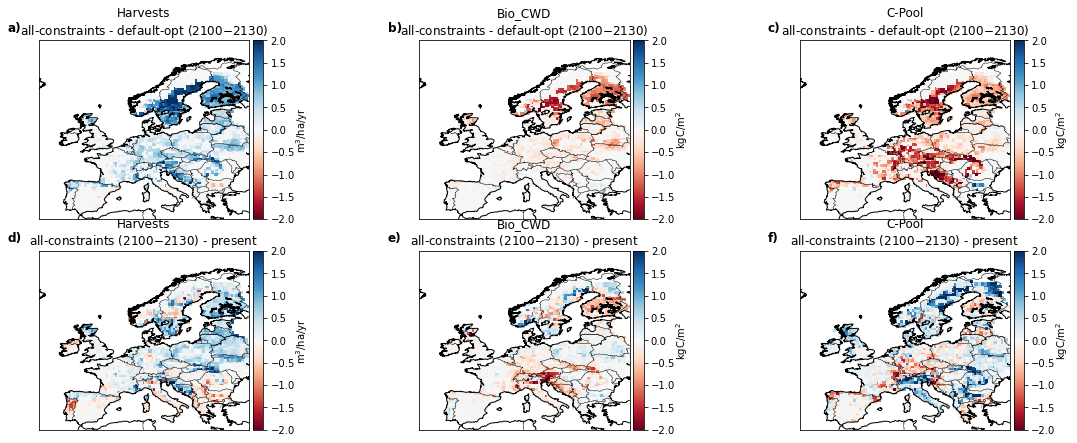
\includegraphics[width=\linewidth]{paper_figs/es_provision_diffs45.png}
	\caption{Comparison of ecosystem service provision between constrained optimization, unconstrained optimization, and present day. Modeled harvest provision (in $\SI{}{\cubic\meter\per\hectare\per\year}$ dry biomass) in the future (2100--2130) for RCP4.5 for \textit{all-constraints} compared to \textit{default-opt} (\textbf{a}) and to present-day (\textbf{d}).
		The same is shown for coarse woody debris (\textbf{b} and \textbf{e}) and the forest carbon pool (vegetation + litter + soil, \textbf{c} and \textbf{f}), in kgC/m$^2$. Similar results were obtained for the other RCPs (Figs. \ref{fig:es-provision-diffs26}-\ref{fig:es-provision-diffs85}).}
	\label{fig:es-provision-diffs}
\end{figure}







%%%%%%%%%%%%%%%%%%%%%%%%%%%%%%%%%%%%%%%%%%%%%%%%%%%%%%%%%%%%%%%%%%%%%%%%%%%%%%%%%%%%%%%%%
%%%%%%%%%%%%%%%%%%%%%%%%%%%%%%%%%%%%%%%%%%%%%%%%%%%%%%%%%%%%%%%%%%%%%%%%%%%%%%%%%%%%%%%%%
%%%%%%%%%%%%%%%%%%%%%%%%%   DISCUSSION
%%%%%%%%%%%%%%%%%%%%%%%%%%%%%%%%%%%%%%%%%%%%%%%%%%%%%%%%%%%%%%%%%%%%%%%%%%%%%%%%%%%%%%%%%
%%%%%%%%%%%%%%%%%%%%%%%%%%%%%%%%%%%%%%%%%%%%%%%%%%%%%%%%%%%%%%%%%%%%%%%%%%%%%%%%%%%%%%%%%


\section{Discussion}


\glsresetall


Our methodology derives multi-functional forestry strategies in Europe under emission scenario uncertainty, providing suggestions for management portfolios that are viable for RCPs 2.6, 4.5, 6.0, and 8.5 simultaneously. While future work will also need to consider uncertainty related to the choice of climate and vegetation model, our results already suggest that constraints on stable harvest levels and protection goals inspired by EU strategies heavily restrict the possibilities to provide other \glspl{es} under climate change.
Furthermore, achieving these targets conflicted with the goal of multi-functionality and with carbon sink targets, complementing findings of previous studies \parencite[e.g.,][]{Blattert2023}.
It is noteworthy that while the EU strategies outline plans for 2030, we examined potential long-term consequences in 2100--2130.



\subsection{Reconciling demands on forest protection, wood production, and mitigation}

The unconstrained \textit{default-opt} optimization indicated that leaving 26\% of currently managed forests untouched benefits multiple \glspl{es} across all RCPs (Fig. \ref{fig:portfolios-original-and-harv}). This exceeds the EU Biodiversity Strategy requirements but implies a drastic reduction in harvests, reducing economic activity and the important role of wood products in climate change mitigation \parencite{Grassi2021, gregorQuantifyingImpactKey2024}.
To maintain current Europe-wide harvest levels we found that inter-regional cooperation is critical, because the harvest constraint could only be met when allowing such cooperation (\textit{min-harv}) and not when it was imposed on every grid cell independently (\textit{min-harv-cell}).
The constraint decreased the proposed shares of unmanaged forests to 5\%, conflicting with strict protection goals (Fig. \ref{fig:portfolios-original-and-harv}).
This was reconciled by the constraint on strict protection (\textit{all-constraints}). However, the burden was not shared equally among regions. Some regions, particularly in the north, had to focus almost exclusively on wood production to compensate for decreased harvests due to strict protection elsewhere. This bears risks for nature protection in those regions (Fig. \ref{fig:unmanaged-cells}b).


Due to climate change, the forest carbon pool declined in many regions (Fig. \ref{fig:es-provision-diffs}f), driven by increased decomposition of litter and soil, especially under higher RCPs. In \textit{default-opt}, this decrease was offset by higher shares of unmanaged forests, which increased vegetation and deadwood pools. In \textit{all-constraints}, however, the carbon pools of the numerous, mainly northern, regions declined compared to present-day values (Fig. \ref{fig:cpool}), conflicting with the EU LULUCF regulation that aims to increase forest carbon uptake in all member states \parencite[Fig. \ref{fig:es-provision-diffs};][]{EU2018LULUCF}.
Maintaining a European forest sink could be imposed as an additional hard constraint in the optimization, but this would further limit management options.
Since from an atmospheric perspective, it is not relevant where the carbon is taken up, LULUCF goals could theoretically be reformulated to allow compensation between states. Although this could facilitate collaboration to achieve the desired atmospheric \coo{} reductions while optimizing other \glspl{es}, this would introduce additional problems of responsibility and accountability.


%Such a necessary development of focus regions for particular ecosystem services have also been suggested by recent studies dealing with ecosystem service provision and timber production in Europe \parencite{Gutsch2018, LessaDerciAugustynczik2021}.
% Gutsch: north and west germany needs to focus on timber, south and central more on habitat and carbon
% Less derci augustzsfsdf: trade-offs between wood production and other ESs in European beech forests.


\subsection{Effect on other ecosystem services, multi-functionality, and the distribution of managed and protected areas}

Applying \textit{all-constraints} strongly reduced the diversity of the portfolios compared to \textit{default-opt} (Fig. \ref{fig:portfolios-harv-constrained-detailed}).
Many portfolios, particularly in Fennoscandia, contained only one or two management options, because there were only few feasible solutions to the constrained optimization. This made it rarely possible to include other management options for risk diversification and for the benefit of other \glspl{es}. At the grid cell level, a balanced provision of \glspl{es} was no longer guaranteed (Figs. \ref{fig:es-provision-all} and \ref{fig:es-provision}), conflicting with the aim of the EU strategies to foster multi-functionality.
For instance, the harvest constraints significantly reduced the amounts of deadwood and large trees in the future, especially in southern Fennoscandia (Fig. \ref{fig:cwd}) where timber production was prioritized to meet the Europe-wide constraint. This poses a significant threat to biodiversity as many species require these habitats \parencite[e.g.,][]{Berg1995}.
This issue was exacerbated by faster decay of deadwood under higher RCPs (Figs. \ref{fig:litter45}+\ref{fig:litter85}).
The performance of other \glspl{es} also declined, showing that focusing on wood production will undermine other \glspl{es} and vice versa, illustrating a clear trade-off.

The regional imbalance of unmanaged sites, with many in the southern regions and few in the rest (Fig. \ref{fig:unmanaged-cells}c), contradicts the goal to protect various ecosystems throughout the continent \parencite{EuropeanCommissionBiodivStrat2020}.
The strictly protected areas in \textit{all-constraints} were mainly allocated to the least productive regions. This would likely bias the assemblage of species benefiting from protection \parencite[see, e.g.,][]{Hamalainen2018}.
To address this, we also constrained the optimization to uniformly distribute the strictly protected areas, but the \textit{all-constraints-protect-cell} optimization was mathematically infeasible. It could be resolved with an at least 5\% reduction in harvests across Europe but portfolios then strongly focused on needle-leaved forests (74\% of all forests). Although a 5\% reduction in harvests might be acceptable given the significant improvement in nature protection in this scenario, promoting managed needle-leaved forests contradicts current scientific evidence and policies targeted at improving forest resilience through mixed forests including broad-leaved species, as discussed below. 


A land-sparing approach, as suggested by the optimization, can have benefits because assigning focus regions for certain targets can help using forests optimally by leveraging regional advantages \parencite{Gutsch2018, LessaDerciAugustynczik2021}.
This does not inherently conflict with multi-functionality, as for instance strictly protected areas can still provide multiple \glspl{es} apart from biodiversity provision, such as water regulation, or local climate regulation.
Our results, however, suggest such a strong segregation that hinders promoting multi-functional forestry, because large regions had to focus on timber provision at the expense of other \glspl{es}.
Even changing the optimization methodology -- affecting how the burden of the constraints could be shared across regions -- had practically no effect on the portfolios (Fig. \ref{fig:sum-vs-minmax}). This further underscores that the constraints heavily limited the forestry options in Europe and that intricate trade-offs need to be made.

Harnessing synergies between different aspects in the same region through land-sharing might be necessary.
In that regard, some biodiversity habitats and other \glspl{es} are compatible with some wood production (e.g., as part of close-to-nature forestry), for instance, by improving landscape-scale heterogeneity, retaining habitat trees and deadwood, and fostering species and structural diversity \parencite[e.g.,][]{Schall2018, Larsen2022, Biber2020, Makela2023}.
Achieving such synergies would help meet wood demands while providing numerous \glspl{es}. 
This approach could make regions that we deemed crucial for timber provision more multi-functional and, with proper measures, also contribute to the 30\% protection target.


The ``triad'' approach aims to combine and enhance land sharing and sparing, by combining intensive and extensive management with strict reserves, based on biodiversity-yield assessments \parencite{Betts2021}.
Nonetheless, while these are desirable approaches to optimally use forest land, they cannot fully resolve the issue of excessive demands imposed on forests that we identified in our simulations. 
Therefore, additional measures are necessary to alleviate pressure on forests, as discussed below.

%As we have shown, there is not a lot of room. The distributino of sharing/sparing strategies, or Triad, needs to be carefully evaluated.



%The fact that in those regions wood production must take precedence to satisfy Europe-wide constraints, a land-sharing approach could be more reasonable than strict protection, as it could offer timber and biodiversity provision at the same time. Nevertheless, this would on the one hand again likely decrease the timber supply, and on the other hand, also some highly productive regions need to be protected because some red-listed species, especially insects, might exclusively inhabit such areas \parencite{Hamalainen2018}. 
%(CITATION: in toms manuscript: Nagel et al. 2017a; Kozák et al. 2021; Mikolas et al. 2021)


Besides protection and multi-functionality, the EU also plans to promote broad-leaved species for their greater resilience \parencite{EUForestStrategy2030}. This transition is encouraged by the scientific literature \parencite{Schwaab2020, Astrup2018, Felton2010, SCHELHAAS2010, HLASNY2021, PARDOS2021}. It was also reflected in \textit{default-opt}, which considered multiple \glspl{es} and a higher vulnerability of needle-leaved forests to disturbances (Fig. \ref{fig:portfolios-original-and-harv}a).
However, the constraints prevented this forest conversion and maintained the dominance of conifers due to their higher wood volumes and suitability for long-lived products \parencite{Eurostat2020}. This would hinder adaptation to climate change, especially in regions where needle-leaved species are projected to suffer more.

An important caveat is that, while we did account for increases in disturbance rates and higher baseline rates for needle-leaved forests, these rates did not depend on the specific species or forest structure. A more realistic representation of disturbances -- especially for spruce monocultures -- would likely decrease the share of needle-leaved forests in the optimized portfolios, making the constraint on harvests for long-lived products harder to meet.


\subsection{Ways forward}

Although further studies should validate our results with model ensembles, our study already highlights the significant challenges of reconciling current forest demands without additional interventions. There are numerous options to address the conflicts that should be considered by future studies and policies:
One potential avenue to alleviate the impact of the constraints is increasing the proportion of wood used for long-lived products.
This involves promoting innovative products made from lower quality wood and smaller diameter trees \parencite[e.g.,][]{RAMAGE2017}.
The otherwise beneficial shift towards more broad-leaved trees also decreases the provision of long-lived wood products, affecting the economy and mitigation. This may be addressed by promoting new products derived from broad-leaved species \parencite[e.g.,][]{Hassan2015}.
Also the increased material wood usage of needle-leaved trees would enable an increased share of broad-leaved species.

However, these measures conflict with Europe's current energy mix. Woody bioenergy plays a crucial role in renewable energy supply, with a significant fraction sourced from primary wood \parencite{EUForestStrategy2030, EUBioenergy2021}. About one-fourth of all roundwood harvests are currently used for fuel wood, providing only 6\% of the gross final energy consumption \parencite{EurostatForRemov2022, ScarlatNicolae2019}.
While increased rates of recycling and end-of-life energy-recovery would help, these rates are already high in many EU countries \parencite{EurostatWaste2023}.
Moreover, renewables like solar and wind offer power densities that are orders of magnitude higher than that of bioenergy \parencite{Smil2015}, making their promotion paramount to meet future energy demands while achieving climate and biodiversity goals for forests.

Projected increases in wood demand are also driven by packaging, single-use products, expansion of living areas, and short lifespans of wood products due to aesthetic reasons \parencite{Hill2022, FAO2022, Bierwirth2015}.
Here, stable harvest levels already required intricate trade-offs, underscoring the need to address these increasing demands.
Our study aligns with broader research highlighting that true sustainability in terms of resource usage, biodiversity, and \glspl{es} necessitates a reduction in demands \parencite[e.g.,][]{Richardson2023, Hickel2020}.
It is also crucial that forest-related actions in Europe avoid an offshoring of impacts \parencite{Berlik2002, Mayer2005}. While the strategies explicitly forbid activities leading to deforestation in other regions of the globe \parencite{EuropeanCommissionBiodivStrat2020}, substantial risks remain \parencite{Cerullo2023, Rosa2023}.
Consequently, concerted efforts are required to balance resource demand and supply within Europe, or to establish frameworks which holistically account for resource footprints and prevent externalizing impacts.

The fact that ``only'' 73\% of the net annual increment is harvested in Europe's wood-supplying forests suggests potential for increased harvesting \parencite{FORESTEUROPE2020}.
Studies have already suggested a necessary intensification of harvests outside of strictly protected areas to compensate for reduced wood supply areas due to protection goals \parencite{PIKKARAINEN2024}. However, this could weaken the ecological benefits of the strategies \parencite{RATY2023}.
Moreover, Europe's felling rates (harvests per forest area) are already high compared to global rates (Fig. \ref{fig:faowoodharvest}) and increasing them has been linked to adverse affects on biodiversity, carbon sequestration, and recreation \parencite{Verkerk2014b, Soimakallio2021, Seppala2019, Schulte2022, Skytt2021, Makela2023}.
Critically, higher felling rates would reduce the buffer between harvests and net annual increment that keeps forests a carbon sink. While increased harvests could offer mitigation benefits through substitution effects, these benefits are likely short-lived \parencite{gregorQuantifyingImpactKey2024, BrunetNavarro2021, Harmon2019}.

Furthermore, the area available for wood supply (currently 75\%) could be increased, but this would conflict with conservation goals. Additionally, many unmanaged forests are in unproductive or inaccessible areas, limiting their wood supply potential \parencite{Verkerk2014b}.
Supporting the ongoing reforestation trend in Europe, endorsed by the EU's plan to plant 3 billion trees by 2030, could alleviate pressure on forests \parencite{FORESTEUROPE2020}. However, it will take decades for these trees to provide timber. Furthermore, it is crucial that biodiversity considerations guide such plantings, e.g., in terms of species selection.



\subsubsection{Uncertainty assessment}
Our methodology derives forest management strategies under deep uncertainty, providing solutions that are viable under all considered climate scenarios.
Further studies should use an ensemble of vegetation models that might consider different processes in different levels of detail to address uncertainty in the projections better.
Additionally, studies with LPJ-GUESS for instance emphasize the importance of using also an ensemble of climate projections from general circulation models as forcing data due to significant variation among them for the same RCP \parencite{Ahlstrom2012}. 
Finally, model parameter uncertainty was not considered here, though for LPJ-GUESS  a smaller impact compared to the uncertainty from environmental data has been suggested \parencite{oberprillerClimateParameterSensitivity2022}.
The advantage of the robust optimization concept is that it can be fed not only with simulations of multiple RCPs, but also with simulations from multiple models and forcings. The outcome would again be one set of portfolios, providing the best options across all RCPs, forcings, and models. 
Also diversity in the aims of decision makers could be included \parencite[e.g.,][]{Knoke2023}. This could be done by including multiple sets of preferences for ecosystems, for instance, with higher importance of water regulation on arid regions.
Including all aspects, however, would pose significant computational challenges.

\subsubsection{Regional strategy development}

We examined how legislative constraints impact the development of future forest management strategies at a coarse, Europe-wide scale. This work establishes a foundation for specific applications: Once general strategies, like broadly allocating protected areas among member states, are outlined, our methodology can be applied at a finer scale. At this level, detailed representation of terrain, soil, forest types, and management practices become crucial \parencite{TURNER1996, TURNER1989, Levin1992}. Thus, in a next step, it may be beneficial to re-integrate fine-scale results into the broader framework, to address scaling issues \parencite{Seidl2013}.

Our optimization can facilitate strategy development for specific regions through more detailed forest simulations. This should include more detailed changes in management regimes (e.g., targeting specific age classes), wood usage patterns, and species selection.
Also age and species composition, landscape heterogeneity and additional biodiversity indicators \parencite[e.g.,][]{Muller2010, Cordonnier2014} should be assessed for estimating conservation values \parencite{Neugarten2024}.

Furthermore, regional objectives and constraints can be included, such as connectivity of protected areas as endorsed by the EU strategies, and minimum reserve sizes to capture natural disturbance regimes (``minimum dynamic area'', \textcite{pickettPatchDynamicsDesign1978}). Additional constraints could include targets for deadwood availability and carbon sinks and constraints for the 30\% (non-strictly) protected areas.

From a computational perspective, we propose a hierarchical approach. Here, we simulated and optimized 2885 grid cells spanning the entire continent. These results can inform assessments on a member-state level. Taking France as the largest EU country as an example, applying our methodology on a $\SI{10}{\square\kilo\meter}$ scale is computationally feasible (i.e., 5400 grid cells). This enables strategy development for individual countries independently which can then guide regional optimizations based on high-resolution data of forest structure, existing old-growth forests, ownership structure, and accessibility, to formulate practical strategies.



\section{Conclusion}
In this study, we combined forest management simulations with robust multi-criteria optimization to develop strategies for multi-functional forests in Europe under climate change. The derived management portfolios are viable for a range of emission scenarios simultaneously, and they reconcile demands for wood production and EU targets for biodiversity protection, climate change mitigation, and ecosystem service provision.
Our approach used simplified management scenarios, moderate constraints, extended time scales, and ignored potential uncertainty from multiple models. 
Nonetheless, our findings already highlight significant conflicts between the various demands placed on European forests, requiring additional measures to alleviate the pressure on forests. They also emphasize the need for coordinated efforts to address the various objectives outlined in EU strategies.
Moreover, our results offer insights that can inform the development of forest management strategies at regional scale.
By incorporating more detailed forest management and wood usage scenarios, along with detailed constraints, our methodology can help investigate how innovative practices may help harmonize or alleviate the conflicting demands on European forests. Our approach offers a tool for the necessary integrated view of conflicting climate, biodiversity, and bioeconomy demands.



%TC:endignore


\subsection*{Acknowledgments}
We acknowledge funding from the Bavarian State Ministry of Science and the Arts in the context of the Bavarian Climate Research Network (bayklif) through its BLIZ project (Grant No. 7831-26625-2017, \url{www.bayklif-bliz.de}). We acknowledge funding from the Forest Value project FORECO and the European Forest Institute (EFI) Networking Fund FORMASAM. KG further acknowledges funding from the VELUX Stifrung (\url{www.veluxstiftung.ch}) and the STEPSEC project of the CDRTerra program of the German Federal Ministry of Education and Research (Grant No. 01LS2102C).
The authors gratefully acknowledge the computational and data resources provided by the Leibniz Supercomputing Centre (\url{www.lrz.de}).
We acknowledge using ChatGPT3.5 to help us with grammar and language editing.
Precisely, we asked it to rephrase parts of our original content for clarity and style.

\subsection*{Author Contributions}
KG, AR, and TN conceived of the study through discussions within the FORECO network. KG implemented changes into the model, developed the constrained optimization framework, ran the simulations and optimizations and drafted the first version of the manuscript. All authors significantly contributed to the interpretations of the results and the manuscript.

%TC:ignore



\printbibliography




%%%%%%%%%%%%%%%%%%%%%%%%%%%%%%%%%%%%%%%%%%%%%%%%%%%%%%%%%%%%%%%%%%%%
%%%%%%%%%%%%%%%%%%%%%%%%%%%%%%%%%%%%%%%%%%%%%%%%%%%%%%%%%%%%%%%%%%%%
%%%%%%%%%%%% FIGURES
%%%%%%%%%%%%%%%%%%%%%%%%%%%%%%%%%%%%%%%%%%%%%%%%%%%%%%%%%%%%%%%%%%%%
%%%%%%%%%%%%%%%%%%%%%%%%%%%%%%%%%%%%%%%%%%%%%%%%%%%%%%%%%%%%%%%%%%%%



\begin{figure}[h!]
	\centering
	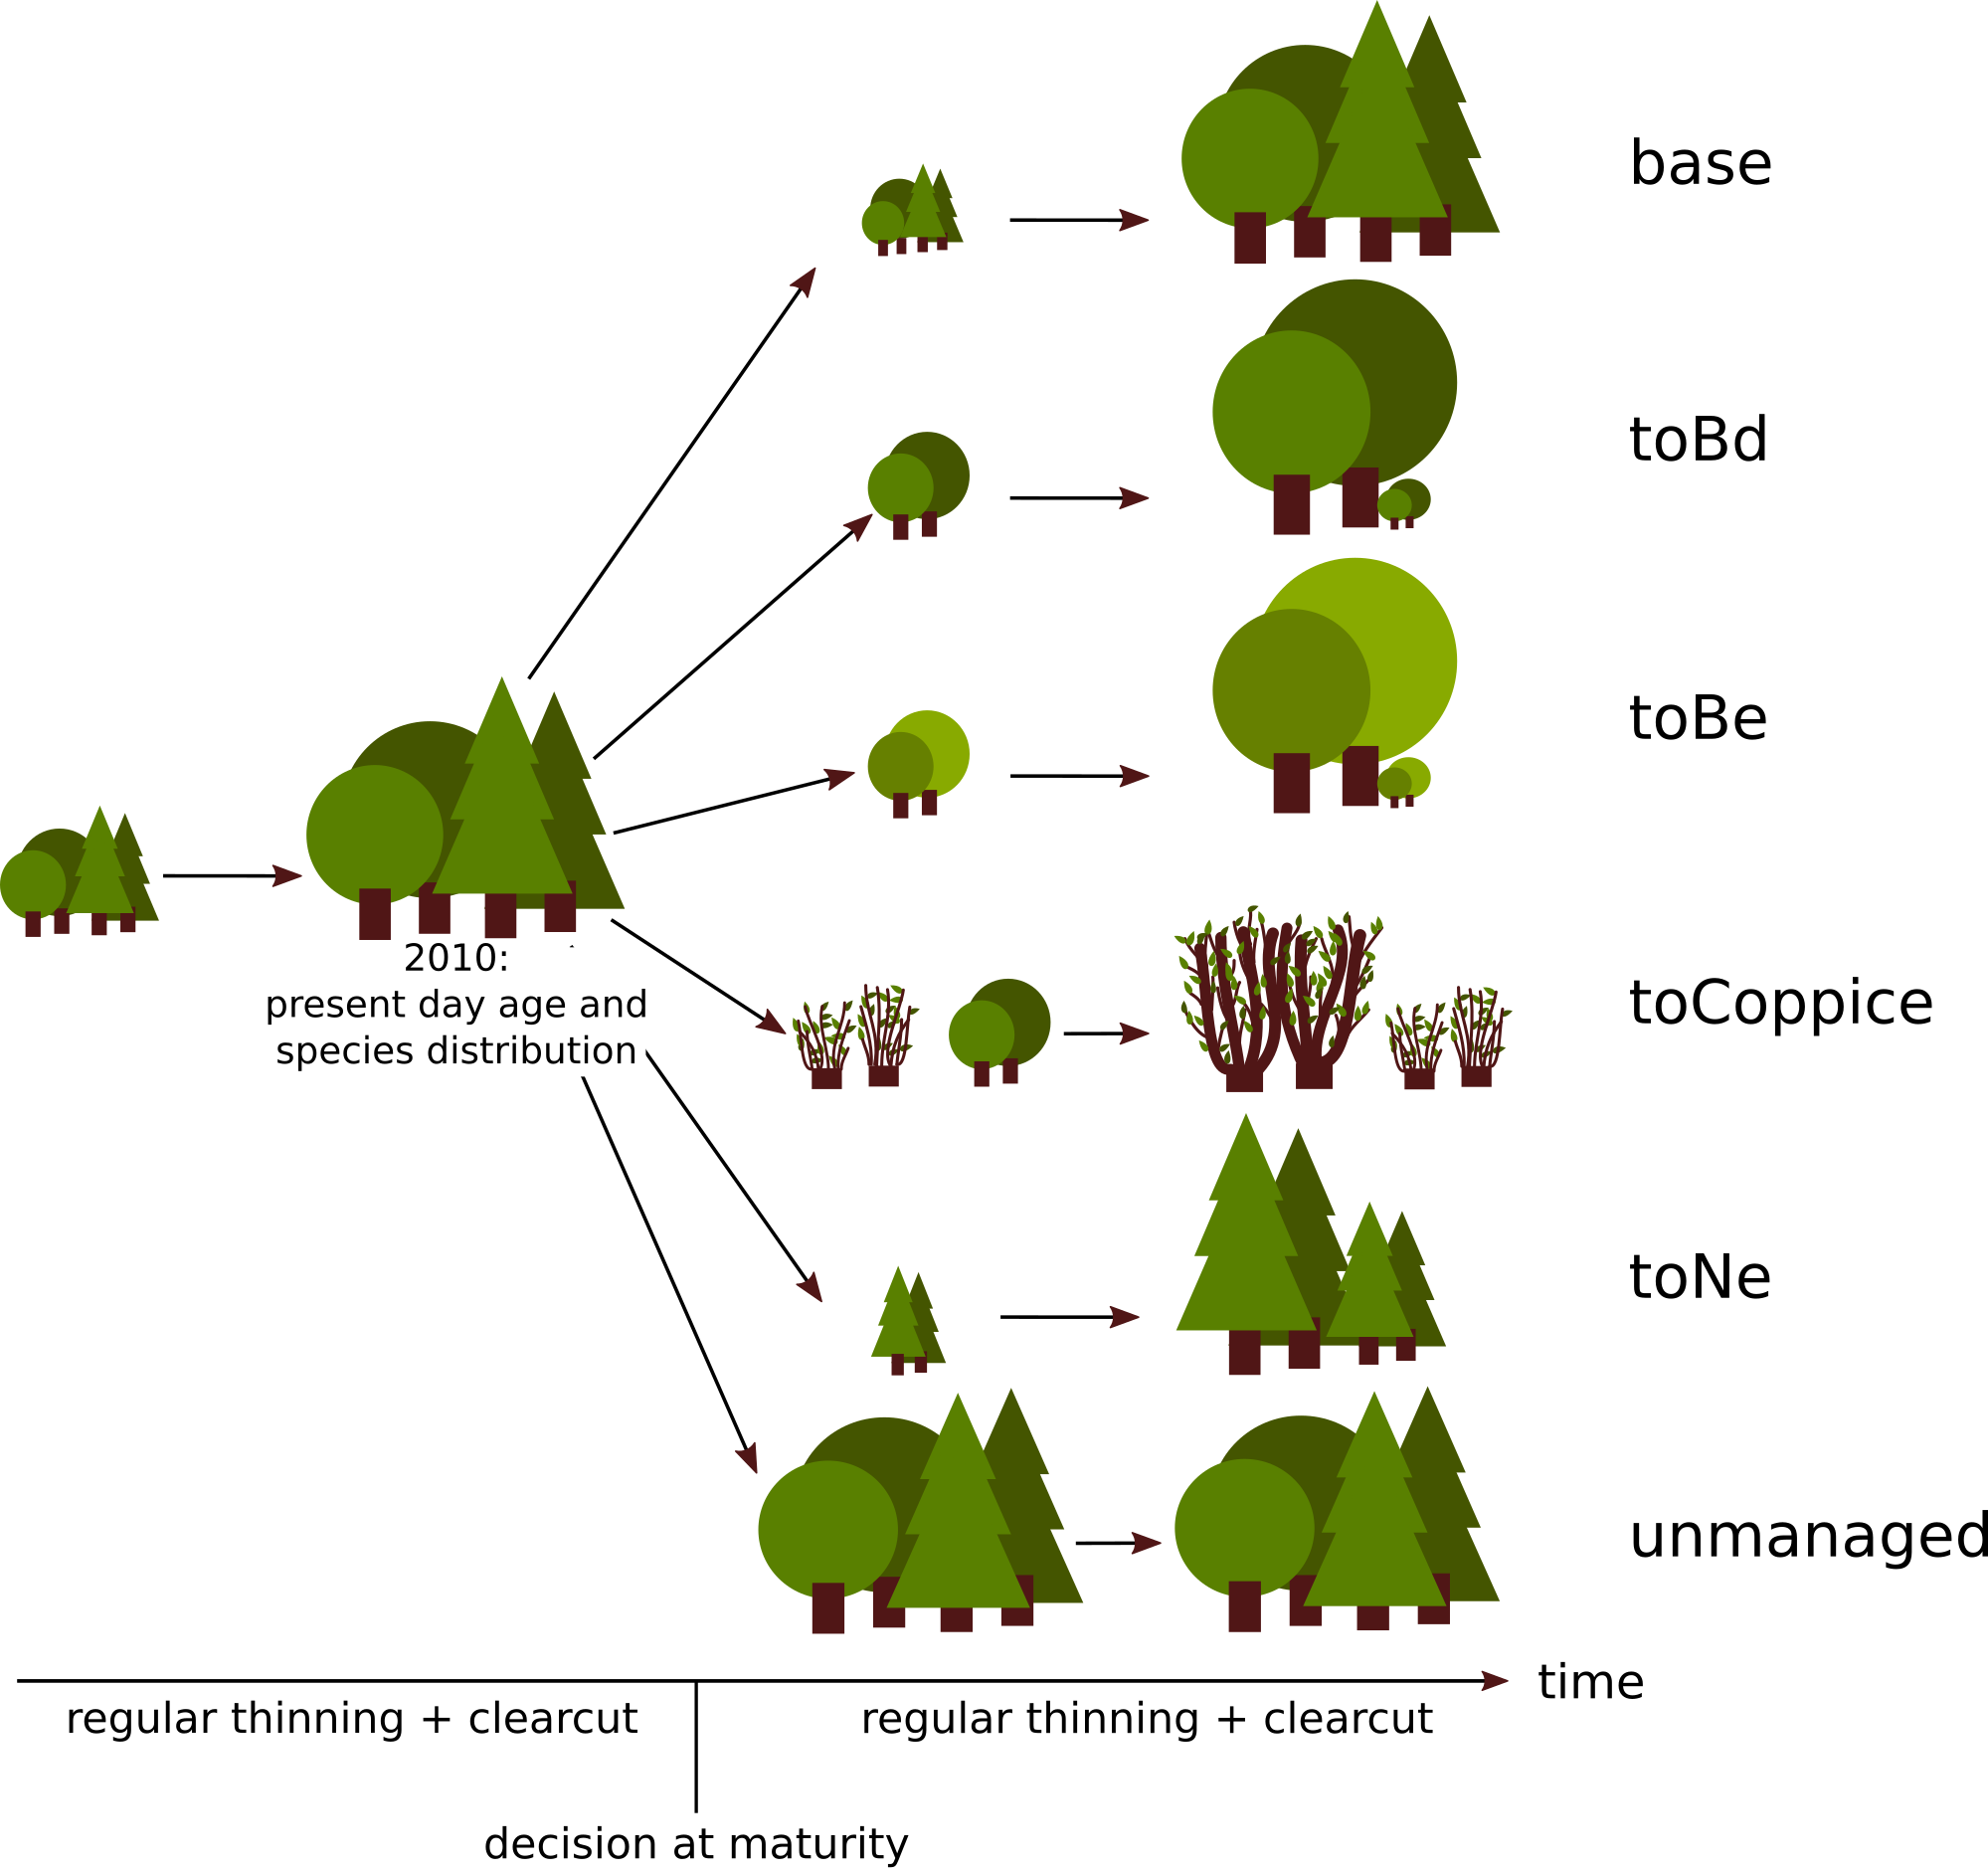
\includegraphics[width=0.5\linewidth]{paper_figs/management_scenarios.png}
	\caption{The six simplified management options, described in section \ref{sec:management-options}. A management decision was made for each stand after 2010 as soon as it reached maturity (i.e. a target density). The conversion was implemented by planting the most common species of each forest type for that grid cell.}
	\label{fig:management}
\end{figure}






\begin{figure}[!h]
	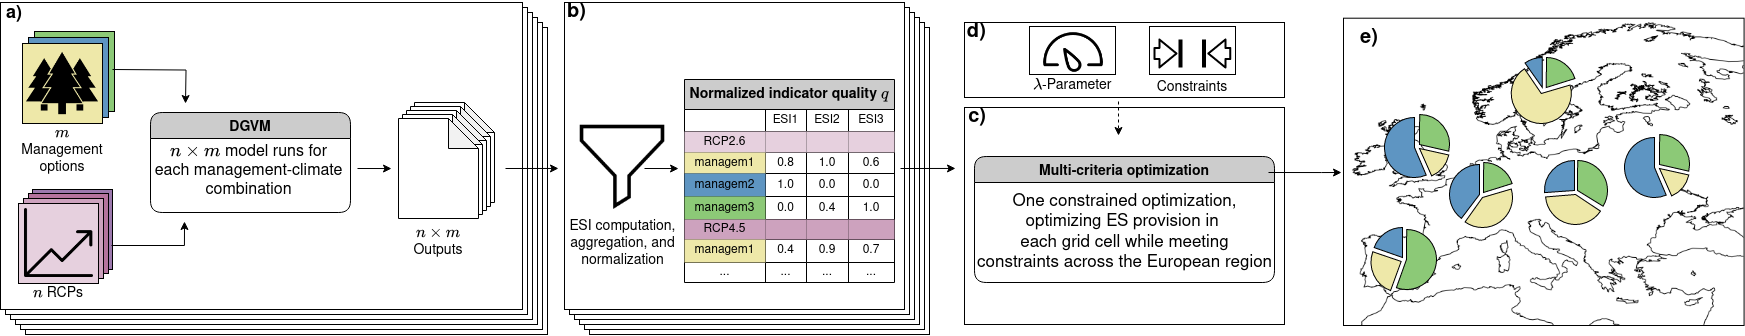
\includegraphics[width=\linewidth]{paper_figs/optimization_newmethod.png}
	\caption{Visualization of the methodology, which computes one collection of portfolios for the entire modeled area. 
		\textbf{a)} For each grid cell, the \textit{m} management options are simulated for the \textit{n} RCPs, resulting in $n\times m$ model simulations. 
		\textbf{b)} ESIs are derived from model outputs, aggregated to the 2100--2130 mean, and normalized. Thus for each grid cell, there was one table containing the normalized values for all RCPs and management options. 
		\textbf{c)} One optimization for all grid cells, configured with Europe-wide constraints (\textbf{d}) computes \textbf{e)} one set of optimized portfolios. Within grid cells, this ensures an optimally balanced provision of all ESIs across all RCPs and that the constraints are met, either on a per-grid-cell basis, or on a Europe-wide level, depending on the nature of the constraint, see section \ref{sec:constraints}.
		\textbf{d)} The parameter $\lambda \in [0, 1]$ specifies the focus on the balanced provision of the ESI. A low $\lambda$ focuses more on a balanced provision of ESIs while a high $\lambda$ improves more the average ESI performance (see section \ref{sec:original-optimization}).
	}
	\label{fig:newoptimization}
\end{figure}





\begin{figure}[h!]
	\centering
	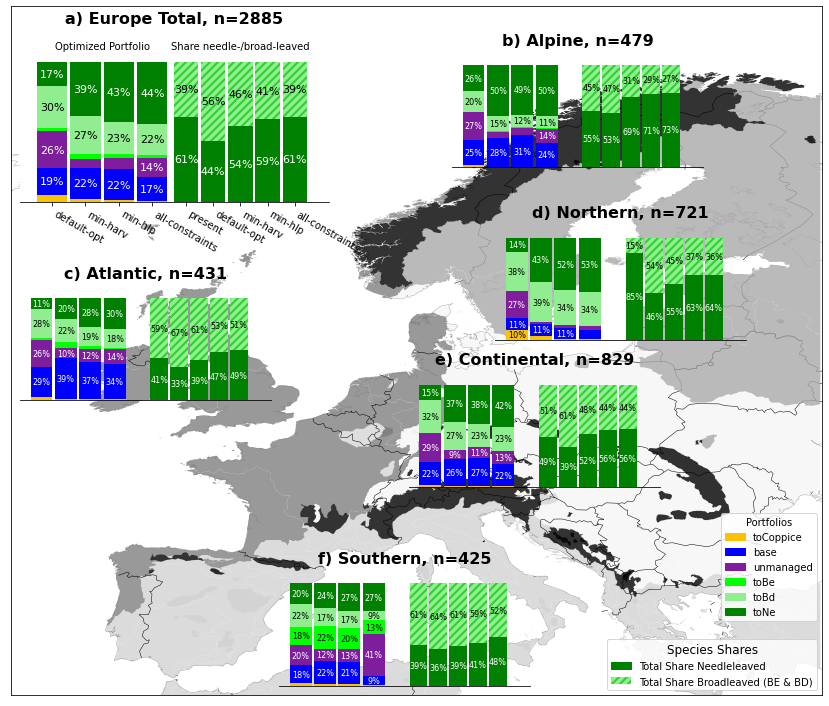
\includegraphics[width=\linewidth]{paper_figs/compare_portfolios_europe_final_revision.png}
	\caption{Portfolios of management options and species shares for optimizations with and without constraints for all of Europe (a) and different European regions (b-f). ``Broad-leaved'' contains broad-leaved evergreen and deciduous species. The six management options are shown in Fig. \ref{fig:management}. Note that the portfolios marginally differed from the results of \textcite{Gregor2022} due to an improvement in the simulation of harvesting and the higher resolution. The number $n$ refers to the modeled grid cells in the given region.}
	\label{fig:portfolios-original-and-harv}
\end{figure}






\begin{figure}[h!]
	\centering
	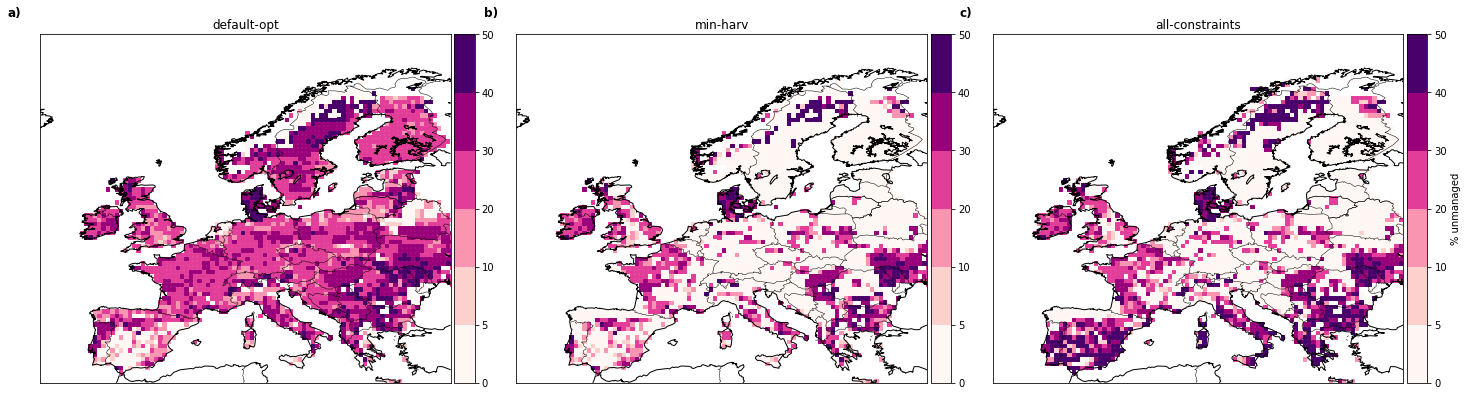
\includegraphics[width=0.9\linewidth]{paper_figs/unmanaged_cells.png}
	\caption{Share of unmanaged forests in \textbf{a)} the default optimization without any constraint, \textbf{b)} when imposing the \textit{min-harv} constraint on harvest levels, and \textbf{c)} when imposing constraints on harvests, harvests for long-lived products, and unmanaged areas at the same time.}
	\label{fig:unmanaged-cells}
\end{figure}




\begin{figure}[h!]
	\centering
	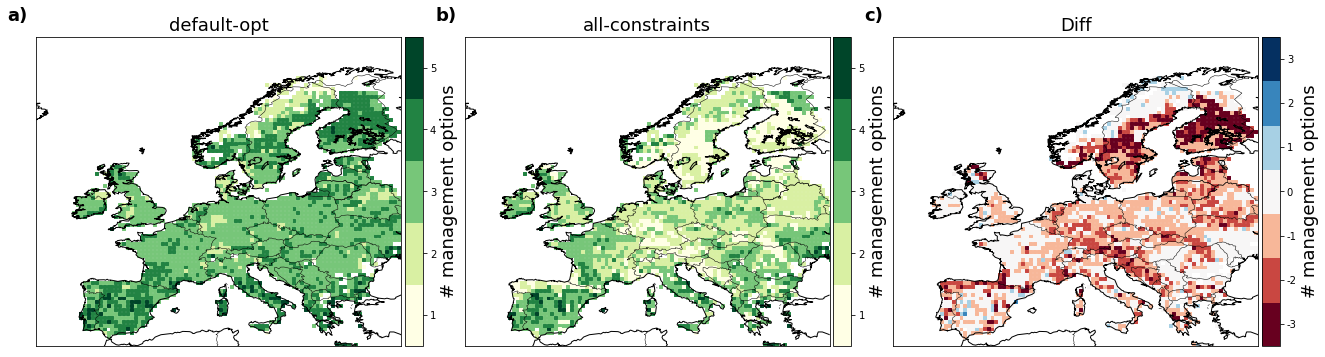
\includegraphics[width=\linewidth]{paper_figs/less_diverse_portfolios.png}
	\caption{Number of management options in the portfolios without constraints (\textbf{a}), and for \textit{all-constraints} (\textbf{b}). \textbf{c}) shows the difference between the two (b-a). Including the constraints led to less diverse portfolios, sometimes even consisting of only one management option, particularly in the Northern region.}
	\label{fig:portfolios-harv-constrained-detailed}
\end{figure}






\begin{figure}[h!]
	\centering
	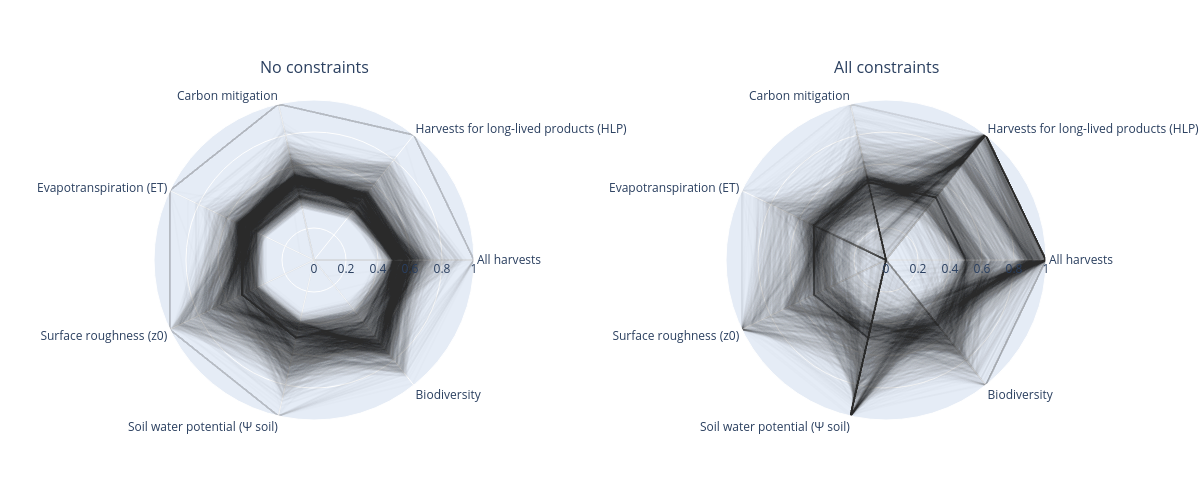
\includegraphics[width=0.8\linewidth]{paper_figs/all_cells_es_provision.png}
	\caption{Provision of ecosystem services across all grid cells. Note that the ecosystem service provision is much more balanced in the unconstrained \textit{default-opt} optimization, i.e. almost all grid cells provide all ecosystem services in a balanced way (\textbf{left}). When imposing \textit{all-constraints}, the provision is much more imbalanced (\textbf{right}). Various cells are required to utilize the maximal possible harvests, affecting also other ecosystem services, often negatively.}
	\label{fig:es-provision-all}
\end{figure}



\begin{figure}[h!]
	\centering
	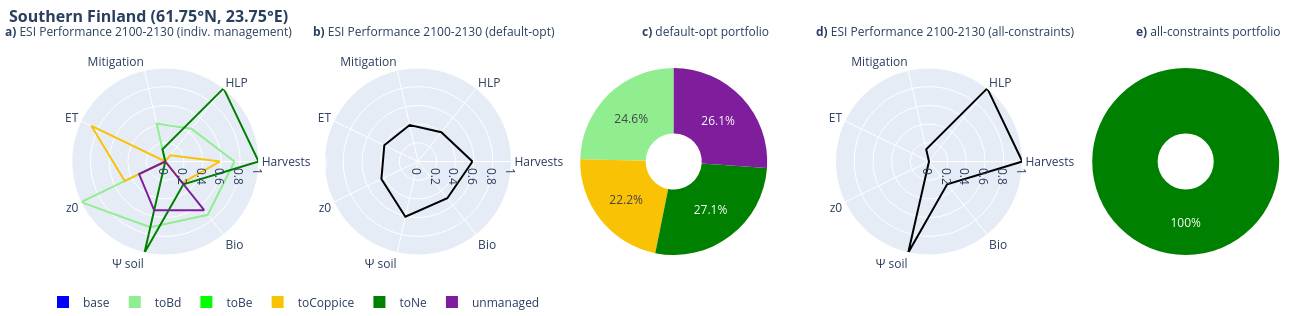
\includegraphics[width=\linewidth]{paper_figs/es_provision.png}
	\caption{Example for a concrete portfolio computed by the methodology for a grid cell in southern Finland. \textbf{a}) shows the ecosystem service provision in the worst case across all RCPs for each management option as measured by the normalized ecosystem service indicators (ESIs). \textbf{b}) shows the worst case ecosystem provision of the optimized portfolio without constraints (\textit{default-opt}) and \textbf{c}) shows the portfolio shares for \textit{default-opt}. \textbf{d}) and \textbf{e}) are like \textbf{b}) and \textbf{c}), respectively, but for \textit{all-constraints}. It is obvious that the ecosystem service provision in \textit{default-opt} is more balanced than in \textit{all-constraints} and that there is no risk diversification in \textit{all-constraints}, as opposed to \textit{default-opt}.}
	\label{fig:es-provision}
\end{figure}





\end{document}
